% Source: inputs/original_04.pdf p.3 (printed 4-35), question 21 figure.
% Representative parameters m=-2/3, p=1/3 satisfy OQ perpendicular OR and p=m^2/(m+2).
% Q=(-(3+sqrt5)/6,(sqrt5-1)/6), R=((sqrt5-3)/6,-(sqrt5+1)/6). No focus F in this figure.
\usetikzlibrary{arrows.meta,calc}
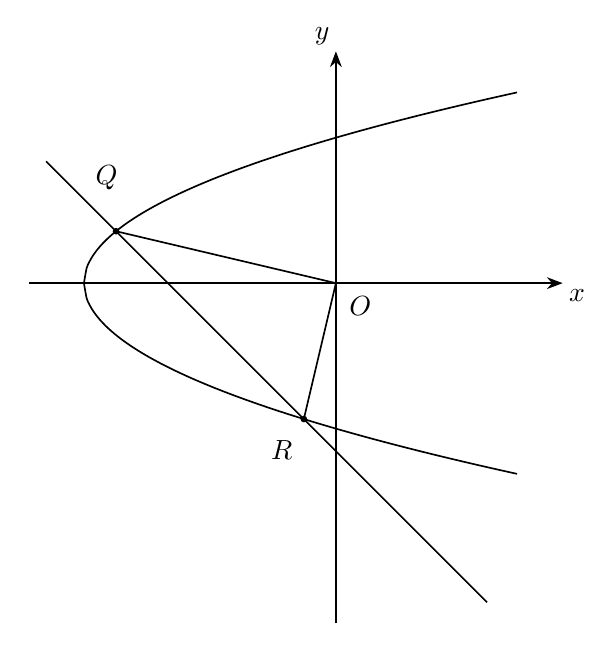
\begin{tikzpicture}[x=3.2cm,y=3.2cm,line width=.6pt,font=\normalsize,>=Stealth]
  \coordinate (O) at (0,0);
  \coordinate (V) at (-1,0);
  \coordinate (Q) at (-0.872678,0.206011);
  \coordinate (R) at (-0.127322,-0.539345);
  \coordinate (L1) at (-1.15,0.483333);
  \coordinate (L2) at (0.60,-1.266667);

  \draw[->] (-1.22,0)--(0.90,0);
  \draw[->] (0,-1.35)--(0,0.92);
  \node[anchor=north west,inner sep=0pt,xshift=2pt,yshift=-2pt] at (0.9,0.0) {$x$};
  \node[anchor=south east,inner sep=0pt,xshift=-2pt,yshift=2pt] at (0.0,0.92) {$y$};

  \draw plot[domain=-1:0.72,samples=161,smooth] (\x,{sqrt((\x+1)/3)});
  \draw plot[domain=-1:0.72,samples=161,smooth] (\x,{-sqrt((\x+1)/3)});
  \draw (L1)--(L2);
  \draw (O)--(Q);
  \draw (O)--(R);

  \fill (Q) circle (1.2pt);
  \fill (R) circle (1.2pt);

  \node[above=5pt,inner sep=1pt] at (-0.91,0.30) {$Q$};
  \node[anchor=north east,inner sep=0pt] at (-0.17,-0.62) {$R$};
  \node[anchor=north west,inner sep=0pt] at (0.05,-0.05) {$O$};
\end{tikzpicture}
